\begin{figure}[h]
    \centering
    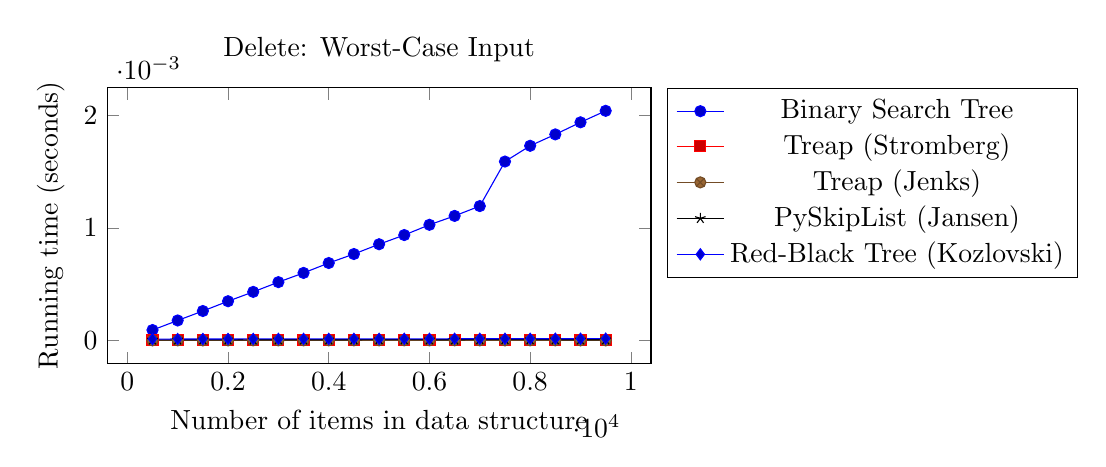
\begin{tikzpicture}
        \begin{axis}[
            xlabel={Number of items in data structure},
            ylabel={Running time (seconds)},
            title={Delete: Worst-Case Input},
            width=0.7\textwidth,
            height=2in,
            legend pos=outer north east
        ]
		\addplot coordinates {
			(9500, 0.0020412429506147765)
			(9000, 0.001939283052110863)
			(8500, 0.0018318899505319487)
			(8000, 0.0017306950373833984)
			(7500, 0.0015906334470270345)
			(7000, 0.0011948499017415592)
			(6500, 0.001107680724025517)
			(6000, 0.001028574010074319)
			(5500, 0.0009375527998012245)
			(5000, 0.000855919224774695)
			(4500, 0.0007689668933011085)
			(4000, 0.0006889506298329274)
			(3500, 0.0006010526078019396)
			(3000, 0.0005191630337391828)
			(2500, 0.00043245766604172787)
			(2000, 0.0003495230135604288)
			(1500, 0.00026249840000602375)
			(1000, 0.00017862106872069462)
			(500, 9.334327211945492e-05)
		};
		\addplot coordinates {
			(9500, 3.6954213819484492e-06)
			(9000, 3.2677524037794115e-06)
			(8500, 2.6443194566994066e-06)
			(8000, 2.3853086670655443e-06)
			(7500, 2.873212712586337e-06)
			(7000, 3.123188242106778e-06)
			(6500, 3.5809747539872206e-06)
			(6000, 3.5267631933422196e-06)
			(5500, 3.7104801487686247e-06)
			(5000, 2.5569786090073875e-06)
			(4500, 3.4454458524280087e-06)
			(4000, 3.4514693591702894e-06)
			(3500, 2.852130439059408e-06)
			(3000, 2.7406955644337925e-06)
			(2500, 3.4605046192481837e-06)
			(2000, 3.243658376810288e-06)
			(1500, 2.466626007979755e-06)
			(1000, 2.8159893986412498e-06)
			(500, 2.788883618336513e-06)
		};
		\addplot coordinates {
			(9500, 1.569123504445713e-06)
			(9000, 1.650440845395451e-06)
			(8500, 1.912463388364927e-06)
			(8000, 1.9726984557166815e-06)
			(7500, 1.6444173386531703e-06)
			(7000, 1.939569168705191e-06)
			(6500, 2.376273406952123e-06)
			(6000, 1.8130755272594001e-06)
			(5500, 2.3943439271789657e-06)
			(5000, 2.0871450837134377e-06)
			(4500, 2.1202743707604554e-06)
			(4000, 2.1684624246276486e-06)
			(3500, 1.9335456619273826e-06)
			(3000, 1.8221107873372944e-06)
			(2500, 2.0178747562482612e-06)
			(2000, 1.710675912747206e-06)
			(1500, 1.5480412309187842e-06)
			(1000, 2.0118512494704534e-06)
			(500, 1.6414055852820297e-06)
		};
		\addplot coordinates {
			(9500, 7.54745393898304e-06)
			(9000, 7.1137614540717205e-06)
			(8500, 7.848629275741814e-06)
			(8000, 8.216063186594624e-06)
			(7500, 8.767214052838313e-06)
			(7000, 8.80034333988533e-06)
			(6500, 6.924020991903035e-06)
			(6000, 7.800441221874622e-06)
			(5500, 8.110651818746817e-06)
			(5000, 8.529285536802433e-06)
			(4500, 7.30350191620488e-06)
			(4000, 7.1679730146811944e-06)
			(3500, 7.27338438256453e-06)
			(3000, 7.7914059617612e-06)
			(2500, 6.3999759059996106e-06)
			(2000, 7.270372629157862e-06)
			(1500, 7.544442185647426e-06)
			(1000, 6.731268776398735e-06)
			(500, 6.580681108019348e-06)
		};
		\addplot coordinates {
			(9500, 1.7085676853909604e-05)
			(9000, 1.643513812652486e-05)
			(8500, 1.6450196893380564e-05)
			(8000, 1.574243485201521e-05)
			(7500, 1.5769540632319946e-05)
			(7000, 1.5778575892433368e-05)
			(6500, 1.5796646412624683e-05)
			(6000, 1.5185260479029238e-05)
			(5500, 1.523043677956082e-05)
			(5000, 1.5046719824134414e-05)
			(4500, 1.5173213465544678e-05)
			(4000, 1.4619050845929848e-05)
			(3500, 1.4576886298804936e-05)
			(3000, 1.4613027339187567e-05)
			(2500, 1.4534721751644497e-05)
			(2000, 1.426065219519046e-05)
			(1500, 1.381792445016572e-05)
			(1000, 1.3579995934165368e-05)
			(500, 1.301077454765931e-05)
		};
        \legend{Binary Search Tree, Treap (Stromberg), Treap (Jenks), PySkipList (Jansen), Red-Black Tree (Kozlovski)}
        \end{axis}
    \end{tikzpicture}
    \caption{Average of 100 operations, benchmarked every 500, starting at 500.}
\end{figure}